\chapter{Introduction} \label{introduction}
This chapter will introduce the problem addressed in this project. 
Previous similar projects as well as the value of this research will also be addressed.

\section{Background and Motivation}

Traditionally the thermal conductivity, otherwise referred to as the $\kappa$-value, of timber is based simply off the EN 1995:1-1-2004 or similar standards.
This research project will aim to obtain the thermal diffusivity of cross laminated SA-Pine timber by further analysing data obtained by S. van der Westhuyzen for his study of the samples' charring rate.

The thermal diffusivity of timber is a unobservable quantity that cannot be measured directly. 
Instead, it is related to measurements of temperature and time through differential models. 
When heat diffusion is calculated using Finite Element methods(TODO:choose which FEM), the process is usually simplified to a linear problem \citep{Fish:2007}. 
Due to the changes in thermal diffusivity of timber with temperature, as can be seen in EN 1995:1-1-2004(pg number T) and Figure \ref{euroK}, the diffusivity cannot be linearly modelled. 
Therefore, the problem lends itself to being analysed by inversion techniques. 
The aforementioned approach will allow us to obtain information about the diffusivity based on the combination of the information assumed prior to measuring, further referred to as the prior, and the measured data. 
Using statistical inversion leads to a probability distribution that provides us with a collection of diffusivity estimates and their corresponding probabilities.

Currently the fire rating of specific timber samples are based on fire tests conducted in a furnace. 
The furnace is kept at increasing temperatures corresponding with the Standard or ISO 834 fire curve as specified in ISO 834 \citet{ISO:1999}.
This process becomes very costly if it has to be repeated every time that timber is used for construction, as timber usage for multiple story construction projects have increased over the past decades. 
This increase is partially due to the sustainability of timber as a construction material: not only is it renewable but it also has a small carbon footprint \citep{Salvadori:2017}.
Obtaining and standardising different thermal diffusivity values for different species of timber, will assist in more accurate modelling.
If modelling accuracy can be increased, the option to use modelling as either confirmation of fire tests or instead of small scale fire test will become more feasible.

	\begin{figure}
	\label{kvalue_fig}
	\centering
	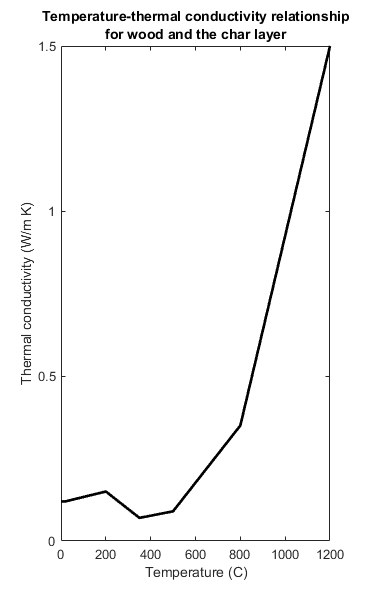
\includegraphics[width = 0.5\linewidth]{figures/kvalues_euro.png}
	\caption{Standard temperature-thermal conductivity relationship for timber from \citep{Euro:2004}}
	\end{figure}/

\section{Aim and objectives}
During the course of the project, the student will aim to meet the following objectives:
\begin{enumerate}
 \item Modify a Finite Element Model into an accurate and effective function;
 \item Compare the model data to the actual acquired data;
 \item Solve for the thermal diffusivity using Bayes' theorem of inverse problems; and
 \item Evaluate and explore the posterior probability distribution using the following methods:
 	\begin{enumerate}
 		\item Maximum a Posteriori
 		\item Markov-Chain Monte Carlo 	
 	\end{enumerate}
\end{enumerate}

\section{Literature study}\label{litstudy}
	
	In their article \textit{Simple Method to Determine the Diffusivity of Green Wood}, \citeauthor{bioresource:2020}  determine the global diffusivity of a Douglas fir green log using inverse identification methods. 
	%In their experiment the also used thermocouples but only 3 at each end.  
	Their experiment was set up by immersing the log with K-type thermocouples into a boiler filled with water at 60$^{^{\circ}}$C. 
	These K-type thermocouples were very specifically placed to improve the accuracy of the diffusivity ratio calculation.
	The finite element model constructed for their calculations used linear interpolation with four node quadrangle elements.
	An analytical model was also constructed using the heat propagation equation(TODO?heat diffusion?).
	The intent of this research was to assist the peeling industry in making the pretreatment process more cost effective.
	The method proved to be effective at determining the thermal diffusivity of green Douglas fir logs, as the $\kappa$-values obtained were comparable to those form literature.
	The methods used by \citet{bioresource:2020} are similar to the methods described later in the report.
	A crucial difference remains as the temperatures at which these experiments were conducted as well as the final usage of the data differ greatly.

%	A similar method of analysis was used by \cite{DeKoker:2021} in their article \textit{Assessment of ice impact load threshold exceedance in the propulsion shaft of an ice-faring vessel via Bayesian inversion}. 
%	Bayesian inversion is used to determine the impact of ice on the propellers from the measurements taken at a specified distance from the propeller. (TODO)

All the thermal properties of various timber species at high temperatures were discussed in an article by \citet{Shi:2021}.

